\section{Introdução}
\hspace{13pt} A busca por um melhor entendimento dos processos e dinâmicas ocorridas na paisagem passa necessariamente por uma melhor compreensão do tempo \citep{gregory85}. 
A aplicação de técnicas de sensoriamento remoto em séries temporais ao longo das últimas décadas contribuíram para que o avanço da detecção de supressões florestais, sejam as relacionados a processos antrópicos, como a processos naturais, fossem utilizadas como subsídio ao desenvolvimento e a aplicação de políticas públicas conservacionistas e restaurativas. Os esforços pelo monitoramento são multi-escalares, mostrando que a aplicação de técnicas de sensoriamento remoto podem ser utilizadas como subsídio a projetos locais \citep{rs12111815}, regionais \citep{Vancutsemeabe1603, silva_junior_brazilian_2021, brandt_unexpectedly_2020}, nacionais \citep{rs12111790} e até mesmo globais \citep{Hansen850, crowther_mapping_2015, POTAPOV2021112165}. A produção desses insumos contribuem diretamente, por exemplo, para o desenvolvimento de cooperações internacionais viáveis foquem em políticas compensatórias visando a redução dos efeitos da mudança climática. 

No entanto, detectar mudanças na paisagem comparando mapas de uso e cobertura a partir de classificações prévias, tendem a propagar erros e a possuírem custo de produção elevado como o caso de projetos governamentais como o realizado pelo IBGE \citep{ibge2020} ou projetos independentes como o Mapbiomas \citep{Souza2019}. O aumento na disponibilidade de imagens prontas para processamento  \citep{rs12030426} em plataformas como o Google Earth Engine facilitaram a aplicação de abordagens que buscam diminuir custos e facilitar o desenvolvimento de produtos no qual o foco pode estar compreendido no entendimento dos processos, sejam eles de curta quanto de longa duração.

Ao longo dos últimos 10 anos algumas soluções começaram a ser desenvolvidas com o intuito de suprir esta demanda. Algoritmos de detecção de mudança em séries temporais como o Landtrendr foram desenvolvidos e aplicados inicialmente em ambientes de florestas temperadas \citep{KENNEDY2012117}. Desde as primeiras versões do algoritmo até hoje, muitas aplicações foram desenvolvidas em diversas áreas como: distúrbios florestais \citep{rs9050479, rs12223720}, mudanças em áreas urbanas \citep{rs12182883, rs13132438}, distúrbios causados por incêndios \citep{rs12091499, rs12233942}, mineração \citep{rs12101612, rs12142235}, distúrbios em áreas de proteção \citep{rs13091800}, detecção de mudanças ou abandonos de áreas de produção agrícola \citep{YIN201812, rs11101234, KOLECKA2021112340, DARA201849}, entre outros.

Alguns trabalhos em âmbito nacional também foram realizados e buscaram aplicar o algoritmo em áreas tropicais com o objetivo de entender seu comportamento em ambientes de maior diversidade ecológica. No entanto, todos os trabalhos focaram em contextos locais ou espacialmente limitados já que só puderam utilizar a primeira versão do algoritmo, ainda desenvolvido em linguagem proprietária IDL e com processamento exclusivo em ambiente offline, o que limitou significativamente a aplicação do mesmo para áreas extensas. O algoritmo foi aplicado primeiramente em áreas de várzea na floresta amazônica \citep{FRAGAL2016} e depois no contexto de Mata Atlântica em escala municipal \citep{Zebende2020} e estadual \citep{Weckmuller2019}. A partir da implementação do algoritmo na plataforma Google Earth Engine \citep{Kennedy2018}, a utilização do mesmo pode ser democratizada e possivelmente ampliada para extensões de terra maiores ao mesmo tempo que diminuiu o custo de produção do mapeamento, já que todo o processamento pesado passou a ser feito de forma gratuita e centralizada em um servidor online.

A partir de sua nova implementação surgiram possibilidades de aplicação do algoritmo visando a detecção de mudanças baseadas em trajetórias não só para paisagens locais como para grandes extensões. No entanto, para que sua aplicação seja de fato difundida como ferramenta de suporte à trabalhos de grande escala e que tenham significância para a elaboração de políticas nacionais e regionais, seria necessário entender seu desempenho quando aplicado a um grande grupo de ecossistemas e diferentes fitofisionomias.

Após análise de diferentes possibilidades de aplicação e áreas de estudo, verificou-se que o bioma da Mata Atlântica poderia ser uma excelente e importante área de estudo para buscar o melhor entendimento da técnica proposta. Assim como sua extensão, o bioma possui outros números impressionantes. É na Mata Atlântica onde cerca de 100 milhões de pessoas vivem e também onde 70\% do produto interno bruto brasileiro é gerado, o que em parte explica o fato de hoje apenas cerca de 12\% de sua cobertura natural ter persistido e apenas 30\% dessas serem protegida em unidades de conservação. Apesar da baixa porcentagem de cobertura natural, é o bioma que abriga mais de 15.700 espécies de plantas e mais de 2.200 espécies de vertebrados registrados pela ciência (260-300 mamíferos; 930-990 aves; 200-300 répteis; 370-480 anfíbios; 300-350 peixes). As estimativas variam, mas, de qualquer forma, impressiona que a Mata Atlântica, representando apenas 0.8\% da superfície terrestre do planeta, abrigue cerca de 5\% das espécies de vertebrados e 5\% da flora mundial. Mesmo tratando-se do bioma brasileiro mais estudado, ainda há muito por se descobrir. Entre 1990 e 2006, registraram-se mais de 1.190 novas espécies de plantas na Mata Atlântica, no coração da área urbana da cidade do Rio de Janeiro e novas espécies são encontradas com alguma frequência. Parte expressiva da fauna e da flora da Mata Atlântica é endêmica, ou seja, não ocorre em nenhum outro lugar do planeta. Estima-se que entre 43\% e 45\% do total de espécies de plantas e vertebrados sejam restritas a esse bioma \citep{scarano2014}.

Sendo assim, o mapeamento se deu em áreas com vegetação de floresta, excluindo áreas de floresta plantada e florestas em ambientes urbanos com o foco de gerar tanto cenários de perda de vegetação quanto de ganho ao longo do período selecionado com o intuito de entender melhor o comportamento do algoritmo na detecção de mudanças para todo o bioma. 

\begin{figure}[h!]
    \centering
    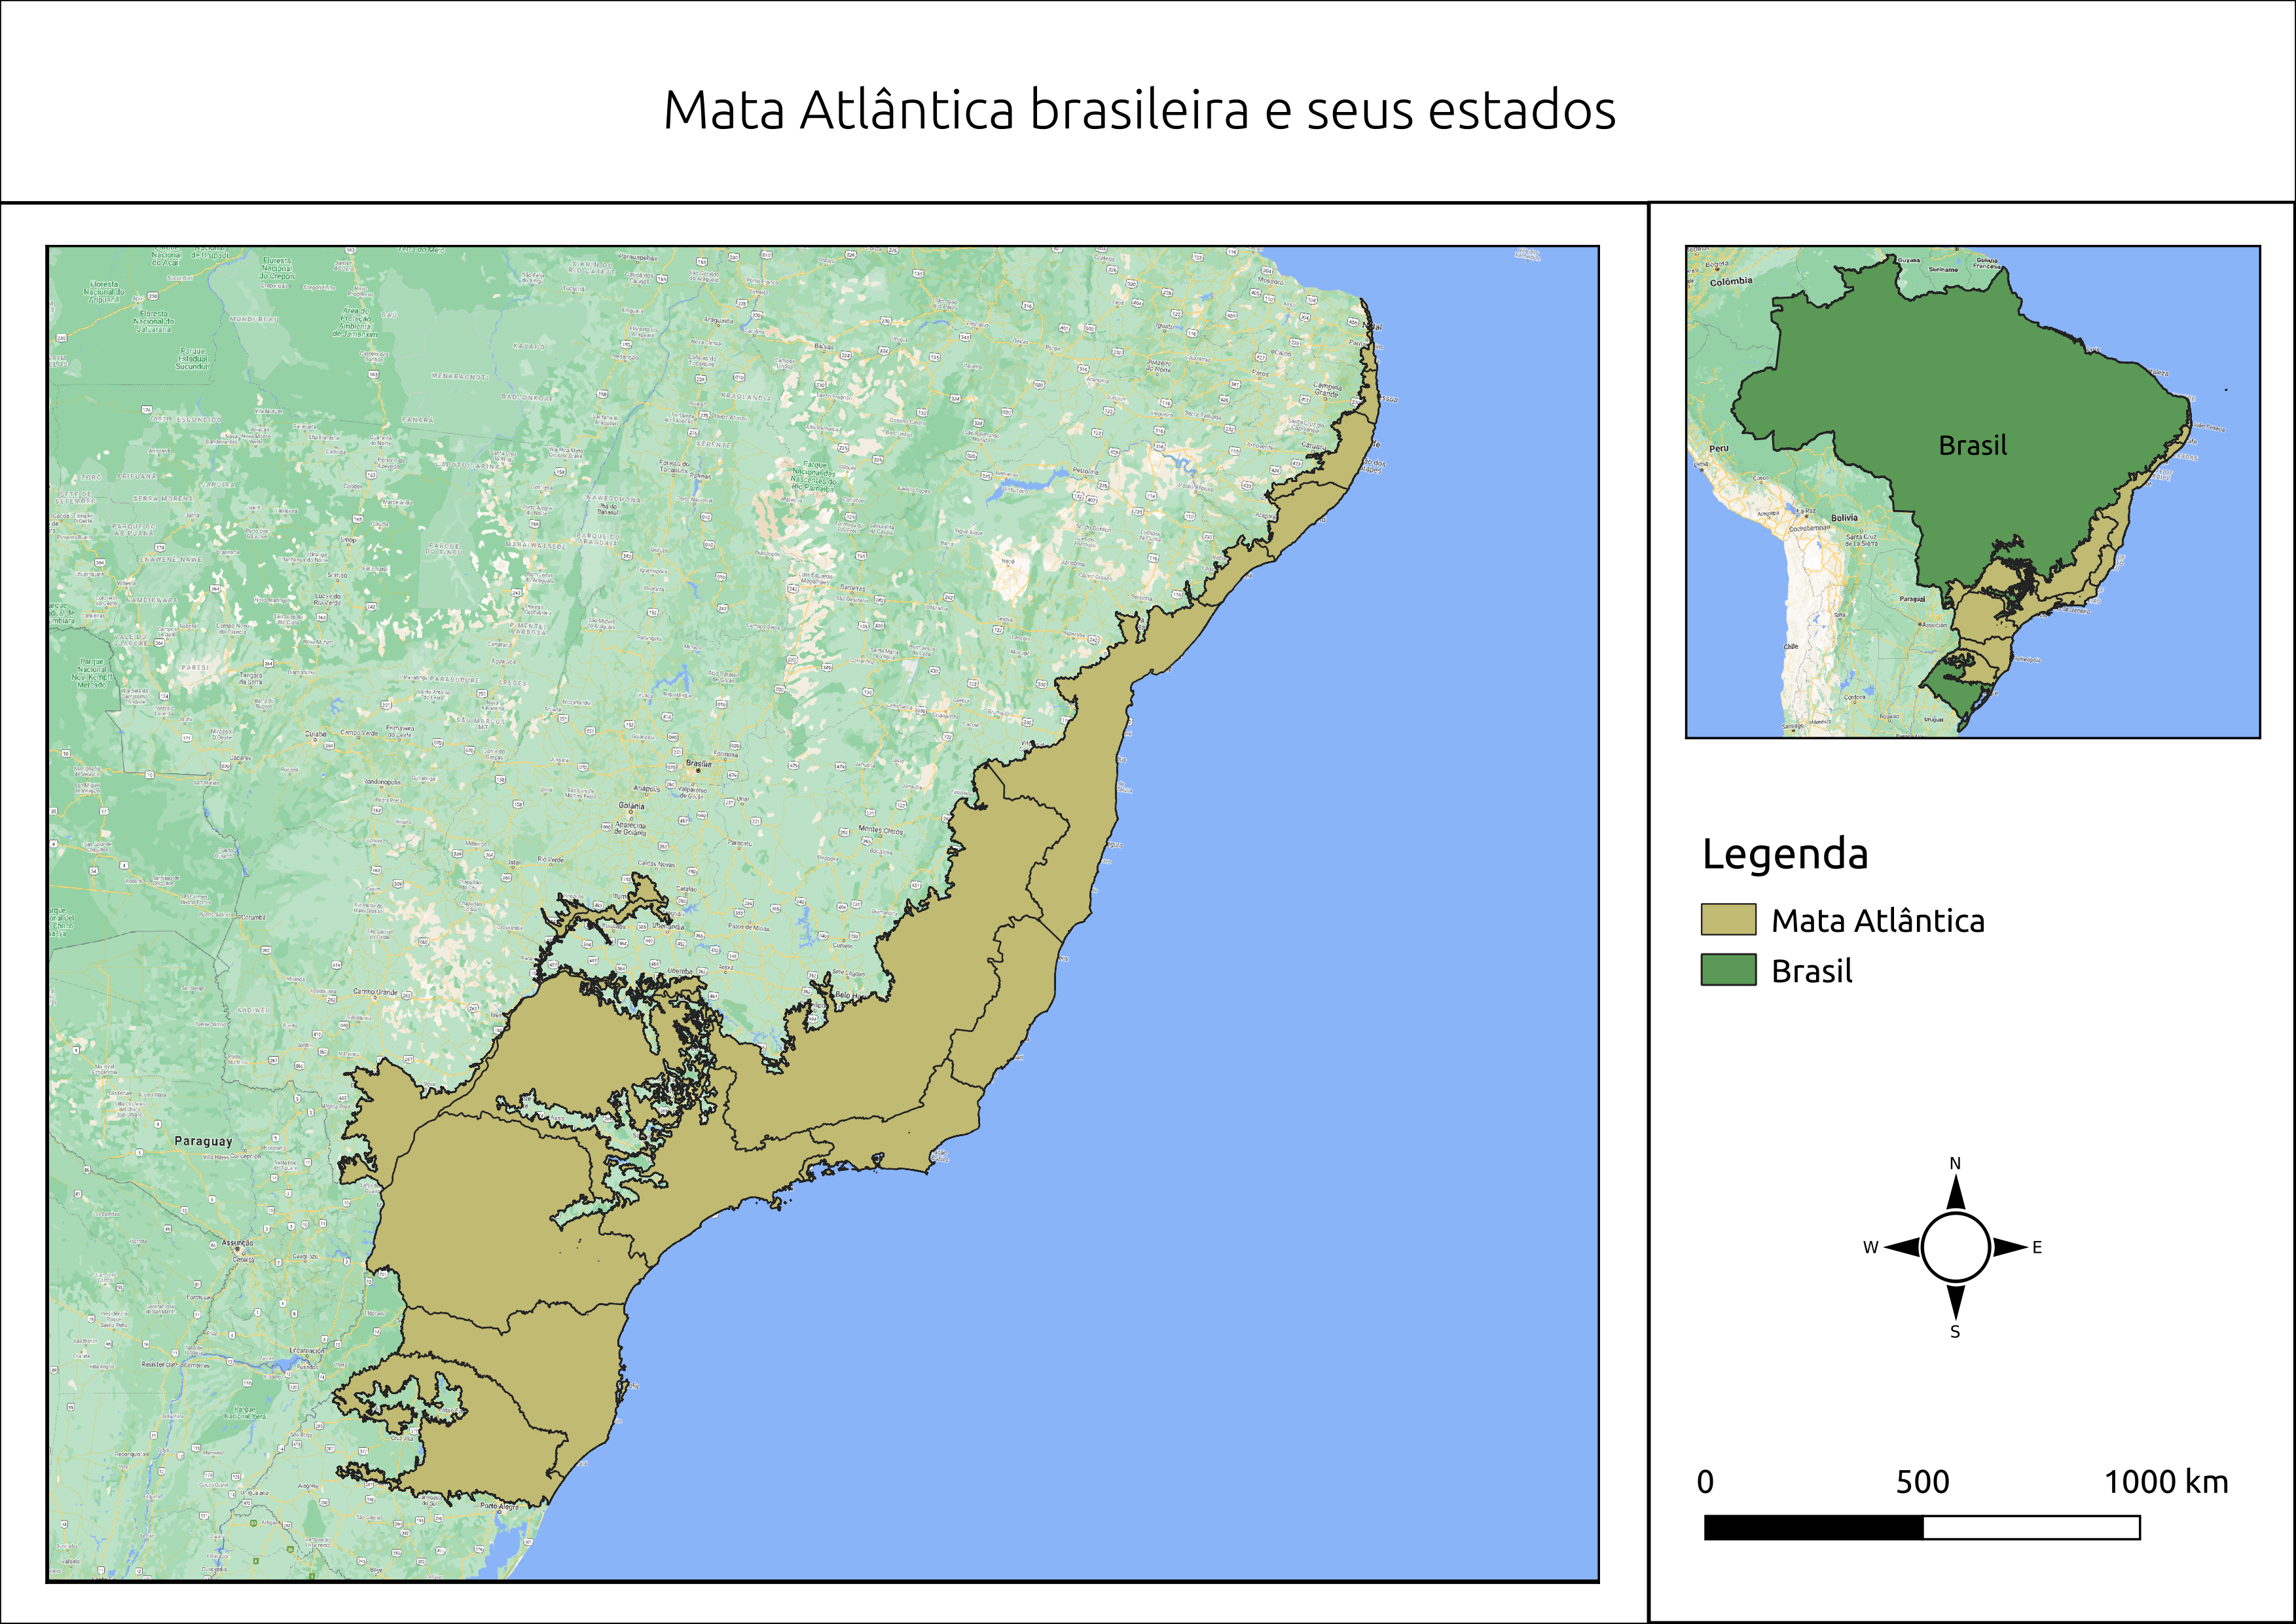
\includegraphics[scale=.5]{images/mata_atlantica.png}
    \caption{Área de Estudo - Mata Atlântica brasileira}
    \label{fig:mata_atlantica}
\end{figure}

\newpage

\subsection{Questionamentos e objetivos da pesquisa}
Os questionamentos motivadores e objetivos da pesquisa foram:
\begin{itemize}
    \item Como um algoritmo como o Landtrendr, inicialmente desenvolvido e utilizado para detecção de mudanças em ambientes de floresta temperada poderia ser utilizado para identificar com alta precisão mudanças ocorridas em uma paisagem complexa como a presente na Mata Atlântica brasileira?
    
    \item O aplicação da metodologia consegue boa performance geral e/ou em diferentes fitofisionomias considerando a aplicação do algoritmo com um mesmo conjunto de parâmetros?
    
    \item Quais as áreas com maior quantidade de perda e ganho de floresta?
    
    \item Como as unidades de preservação existentes da Mata Atlântica se comportaram ao longo dos anos? (ex. Parque Nacional da Serra da Bocaina, Parque Nacional da Serra dos Órgãos, etc)
    
    \item Como os estados e municípios se comportaram ao longo da série temporal? Quais deles ganharam mais do que perderam floresta?
    
    \item Quais os anos com maior quantidade de perda e ganho de floresta?
    
    \item Quais as áreas com maior taxa de mudança tanto para perda como ganho de vegetação? 
    
    \item Qual a idade das florestas secundárias do bioma? 
\end{itemize}

\subsection{Objetivos Específicos}
\begin{itemize}
    \item Definição do período, seleção das imagens e criação da composição da série temporal Landsat a ser utilizada;
    
    \item Compatibilização das imagens utilizadas de acordo com características geométricas e radiométricas com o intuito de evitar possíveis ruídos;
    
    \item Definição dos parâmetros e do índice espectral para a execução do processo de segmentação temporal utilizando o algoritmo Landtrendr;
    
    \item Desenvolvimento do código na plataforma Google Earth Engine para a execução do algoritmo em todas as cenas que englobam o bioma da Mata Atlântica brasileira;
    
    \item Mapeamento das trajetórias florestais compatível com a escala 1:100.000 através da criação de mapas de detecção de magnitude, ano de início da mudança, duração e taxa de mudança;
    
    \item Conversão dos dados matriciais gerados em dados vetoriais com intuito de identificar áreas com maior nível de ocorrência de perdas e ganhos de acordo com divisões políticas e geoecológicas;
    
    \item Mapeamento da idade da floresta secundária;
    
    \item Avaliação da acurácia dos produtos gerados. Avaliar o desempenho do algoritmo em ambientes de florestas tropicais com alto nível de complexidade ecológica.
\end{itemize}